% mycsrf 'for beeing included' snippet template
%
% (c) Karsten Reincke, Frankfurt a.M. 2012, ff.
%
% This text is licensed under the Creative Commons Attribution 3.0 Germany
% License (http://creativecommons.org/licenses/by/3.0/de/): Feel free to share
% (to copy, distribute and transmit) or to remix (to adapt) it, if you respect
% how you must attribute the work in the manner specified by the author(s):
% \newline
% In an internet based reuse please link the reused parts to mycsrf.fodina.de
% and mention the original author Karsten Reincke in a suitable manner. In a
% paper-like reuse please insert a short hint to mycsrf.fodina.de and to the
% original author, Karsten Reincke, into your preface. For normal quotations
% please use the scientific standard to cite
%


%% use all entries of the bibliography

\subsection{MuseScore ($\bigstar\bigstar\bigstar\bigstar\bigstar$)}

\parpic(1cm,1cm)[r][t]{
\includegraphics[width=1cm]{logos/musescore-300dpi.png}}
\label{MuseScore}\acc{MuseScore} bezeichnet sich selbst als das
\enquote{beliebteste Notensatzprogramm der Welt} und verspricht
\enquote{wunderschöne Notenblätter erzeugen, drucken und wiedergeben} zu
können.\footcite[vgl.][\nopage wp]{MuseScore2019a} Erst seit Dezember 2018 gibt
es die Version 3.\footnote{$\rightarrow$
\href{https://musescore.org/en/handbook/developers-handbook/release-notes/release-notes-musescore-3}
{https://musescore.org/en/handbook/developers-handbook/release-notes/release-notes-musescore-3}}
LTS-Distributionen -- wie Ubuntu 18.04 -- werden also noch mehr oder minder
lange die ältere Version 2 mitliefern.\footcite[vgl.][\nopage
wp]{UbuntuMuseScore2018a} Als GPL lizenziertes Open-Source-Software existiert
selbstverständlich auch ein Repository, wo man den entsprechenden Quelltext
herunterladen kann.\footnote{\cite[vgl.][\nopage wp]{GithubMuseScore2019a}. Das
Repository enthält die GPL-2.0 unter dem Dateinamen \texttt{LICENSE.GPL}. Das
Programm ist also freie Software.} Für beide Releases steht je ein
Online-Handbuch zur Verfügung, für \acc{MuseScore2}
ebenso\footcite[vgl.][\nopage wp]{MuseScore2019c}, wie für
\acc{MuseScore3}.\footcite[vgl.][\nopage wp]{MuseScore2019d} Die korrespondieren
PDF-Versionen stellt jedoch nicht \acc{MuseScore} selbst zum Download bereit,
sondern das \acc{Open Source Lab} der \acc{Oregon State University}.\footnote{
$\rightarrow$ \href{http://osuosl.org/}{http://osuosl.org/}} Insofern ist es
völlig korrekt, wenn die PDF-Version-2\footcite[vgl.][\nopage
wp]{MuseScore2019h} und die PDF-Version-3\footcite[vgl.][\nopage
wp]{MuseScore2019g} des \acc{MuseScore}-Handbuches 'nur' über eine 'Fremd-URL'
erreichbar sind. Neben diesen Handbüchern gibt es noch
Video-Tutorials\footcite[vgl.][\nopage wp]{MuseScore2019e} und textuelle
'HowTos' zu speziellen Themen.\footcite[vgl.][\nopage wp]{MuseScore2019f}
Insgesamt ist \acc{MuseScore} damit wohl das am Besten dokumentierte freie
Notensatzprogramm.

Vom Typ her gehört \acc{MuseScore} zu den graphischen Frontends:
hier setzt man Noten visuell, anstatt sie textuell zu editieren. Allerdings
bringt \acc{MuseScore} auch sein eigenes Backend mit, will sagen: seine eigene
'Notensatzmaschine'. Es hängt also nicht von \acc{ABC}, \acc{LilyPond} oder
\acc{MusiX\TeX}\ ab. Insofern darf man es in der Tat als ein integriertes
Gesamtsystem bezeichnen.

Eine weitere Besonderheit bietet \acc{MuseScore} in Sachen Download und
Installation: Natürlich kann man auch die Version nutzen, die die je eigene
Distribution mitbringt. Das wird von Zeit zu Zeit aber nicht die aktuellste
Version sein. Diese aus den Quellen heraus zu kompilieren und zu installieren,
ist ebenfalls möglich, wenn auch ungleich aufwendiger. \acc{MuseScore} will hier
eine Brücke zwischen gepflegtem System und Aktualität schlagen. Deshalb bietet
es \acc{AppImages} zum Download an.\footcite[vgl.][\nopage wp]{MuseScore2019b}
Sie sind deutlich größer als normale Binärpakete, enthalten dafür aber in sich
alle Module, Bibliotheken und Dateien, die benötigt werden.
Solche \acc{AppImages} können daher auch auf Sticks installiert und von Rechner
zu Rechner getragen werden, ohne das Hostsystem erweitern zu
müssen.\footcite[vgl. dazu][\nopage wp]{Prakash2018a} Das einzige, was dabei zu
beachten ist, ist der Typ des Betriebssystems.\footnote{Die folgenden Analysen
haben wir mit MuseScore2 erstellt. Die Ergebnisse können direkt auf MuseScore3
übertragen werden.}

\acc{MuseScore} vermag u.a. \acc{MusicXML}-, \acc{MIDI}- und seine eigene
\acc{MSCZ}-Dateien einzulesen. Bei Fremdformaten geht damit implizit ein
konvertierender Import einher. Umgekehrt kann \acc{MuseScore} seine Musikstücke
-- außer in verschiedenen Audioformaten -- als \acc{MusicXML}-, \acc{MIDI}- oder
Graphikdatei sichern.\footnote{als \acc{PDF}-, \acc{PNG}- oder \acc{SVG}-Datei}
Der Im- oder Export von \acc{ABC}-, \acc{LilyPond}- oder \acc{MusiX\TeX}-Dateien
wird nicht angeboten.\footnote{MuseScore bietet zwar ein \acc{ABC Import plugin}
an ($\rightarrow$ \href{https://musescore.org/en/project/abc-import}
{https://musescore.org/en/project/abc-import} RDL.: 2019-02-21). Dieses Plugin
nutzt allerdings den ABC2XML-Onlinekonverter und liest dann 'nur' den extern
generierten \acc{MusicXML}-Text ein. Insofern handelt es sich dabei um ein
Hybridsystem, das von einer funktionierenden Internetverbindung abhängig ist.}
Damit scheint \acc{MuseScore} auf den ersten Blick recht isoliert dazustehen. Es
gibt allerdings eine Untersuchung vom 'Konkurrenzsystem' \acc{Denemo}, die die
erfolgreiche Übertragung per \acc{MIDI}- und \acc{MusicXML}-Datei anhand eines
sehr komplexen Notentextes nachweist.\footcite[vgl.][\nopage wp]{Denemo2019a}

\acc{MuseScore} kann den Musikanteil unser Referenzdatei II problemlos erfassen:

\begin{center}
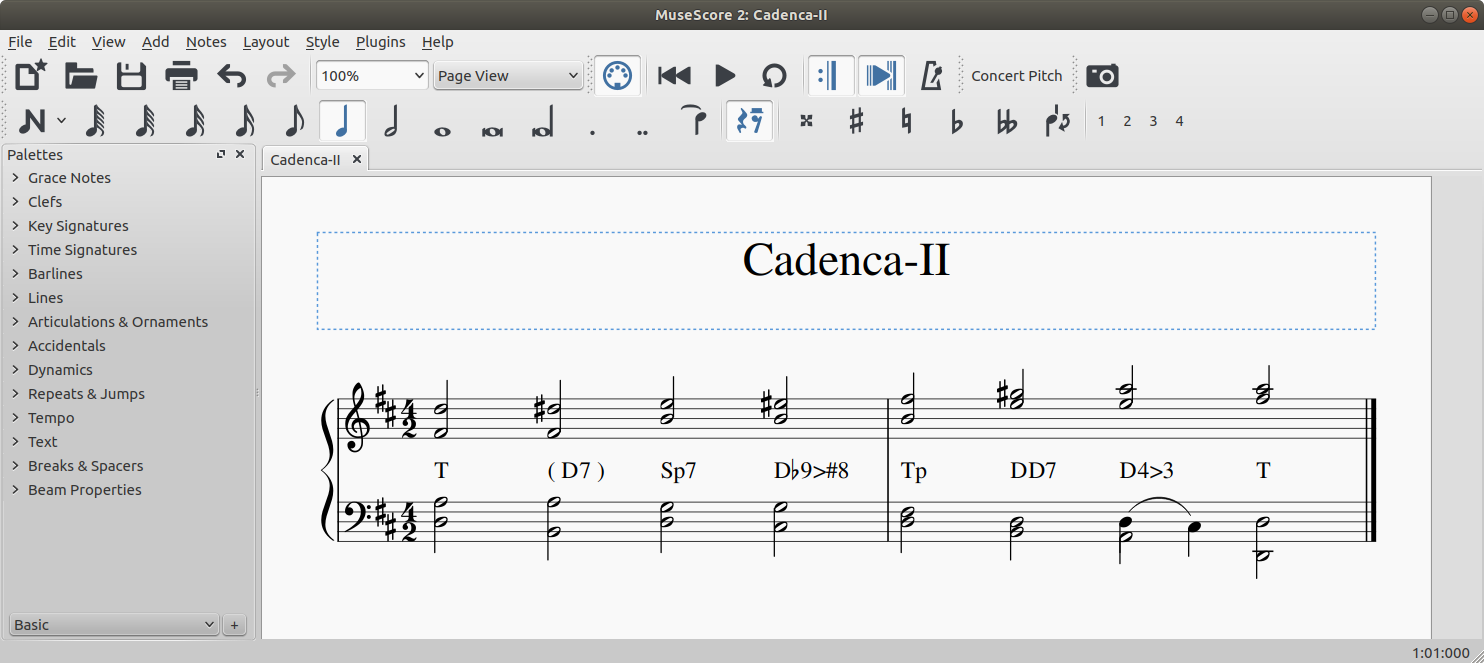
\includegraphics[width=0.9\textwidth]{frontends/musescore/cadenca2-musescore-300dpi.png}
\end{center}

Für die Darstellung von Akkordsymbolen bietet das Programm ein eigens darauf
ausgelegtes System: Man klickt zuerst eine Note in einem System an und tippt
dann \texttt{STR K}. Daraufhin wird über der Note ein Textfeld geöffnet, in das
man seine Symbole eingeben kann. \texttt{b} und \texttt{bb} bzw. \texttt{\#} und
\texttt{\#\#} werden darin musikalisch als (doppelte) Alterationen
interpretiert. Unglücklicherweise erlaubt dieses System jedoch nur die linerare
Aneinandereihung von Zeichen.\footcite[vgl.][\nopage wp]{MuseScore2019i} Eine
zweidimensionale Darstellung komplexer Symbole, wie sie die Funktionstheorie
erwartet, ist damit leider ausgeschlossen.

\acc{MuseScore} bietet ein 'Wohlfühl'-Frontend der Extraklasse. Auch wenn man
sich einarbeiten muss, findet man hier ohne große Anstrengungen, was man als
Musiker sucht, nämlich die Möglichkeit, Noten visuell als Noten zu schreiben.
Die optische Qualität des generierten Notentextes -- am Bildschirm und in den
PDF-Dateien -- ist ebenfalls herausragend. 

Für den Musikwissenschaftler kommt \acc{MuseScore} trotzdem nicht als das
alleinige 'Allheilmittel' in Frage, jedenfalls dann nicht, wenn er die
Standardsymbole in seiner Arbeit verwenden will. In diesem Fall  wird seine
Notenbeispiele zuletzt doch als \acc{MusicXML-} oder \acc{MIDI}-Datei
exportieren und über \acc{LilyPond} oder  \acc{MusiX\TeX}\ um akzeptable
Harmonieanalysen erweitern müssen, bevor er das Ergebnis in seine \LaTeX-Texte
einbettet. Darf er sich dagegen -- aus welchen Gründen auch immer -- mit den
gegebenen Möglichkeiten zufriedengeben, kann er seine Ergebnisse auch als
Graphiken sichern und über diese über die Standardmethode in seine Arbeiten
integrieren.\footnote{$\rightarrow$ S. \pageref{IncludeGraphics}}

Insgesamt aber ist klar, dass MuseScore fünf Sterne verdient: ein
ausgezeichnetes freies graphisches Notensatzprogramm.
% this is only inserted to eject fault messages in texlipse
%\bibliography{../bib/literature}
